% Prevent this chapter being added to the TOC, then add it manually. 
% Otherwise the TOC is weirdly formatted.
\addtocontents{toc}{\protect\setcounter{tocdepth}{-1}}
\chapter[Appendix A]{\phantom{X}}
\addtocontents{toc}{\protect\setcounter{tocdepth}{\sectiontocdepth}}
\addcontentsline{toc}{chapter}{Appendix A}
\labch{appendixA}

% \renewcommand*{\thesubsection}{\Alph{subsection}}
\hspace{0pt}
\vfill
\begin{fullwidth}
    \section{Supplementary figures: Ciliary chemosensitivity is enhanced by cilium geometry and motility}
\end{fullwidth}
\vfill
\hspace{0pt}



\includepdf[pages={4,6}]{pdfs/elife-66322-figures-v2.pdf}


% As with the previous appendix
\addtocontents{toc}{\protect\setcounter{tocdepth}{-1}}
\chapter[Appendix B]{\phantom{X}}
\addtocontents{toc}{\protect\setcounter{tocdepth}{\sectiontocdepth}}
\addcontentsline{toc}{chapter}{Appendix B}
\labch{appendixB}

\hspace{0pt}
\vfill
\begin{fullwidth}
    \section{Supplementary information: Nonreciprocal interactions give rise to fast cilium synchronisation in finite systems}
\end{fullwidth}
\vfill
\hspace{0pt}

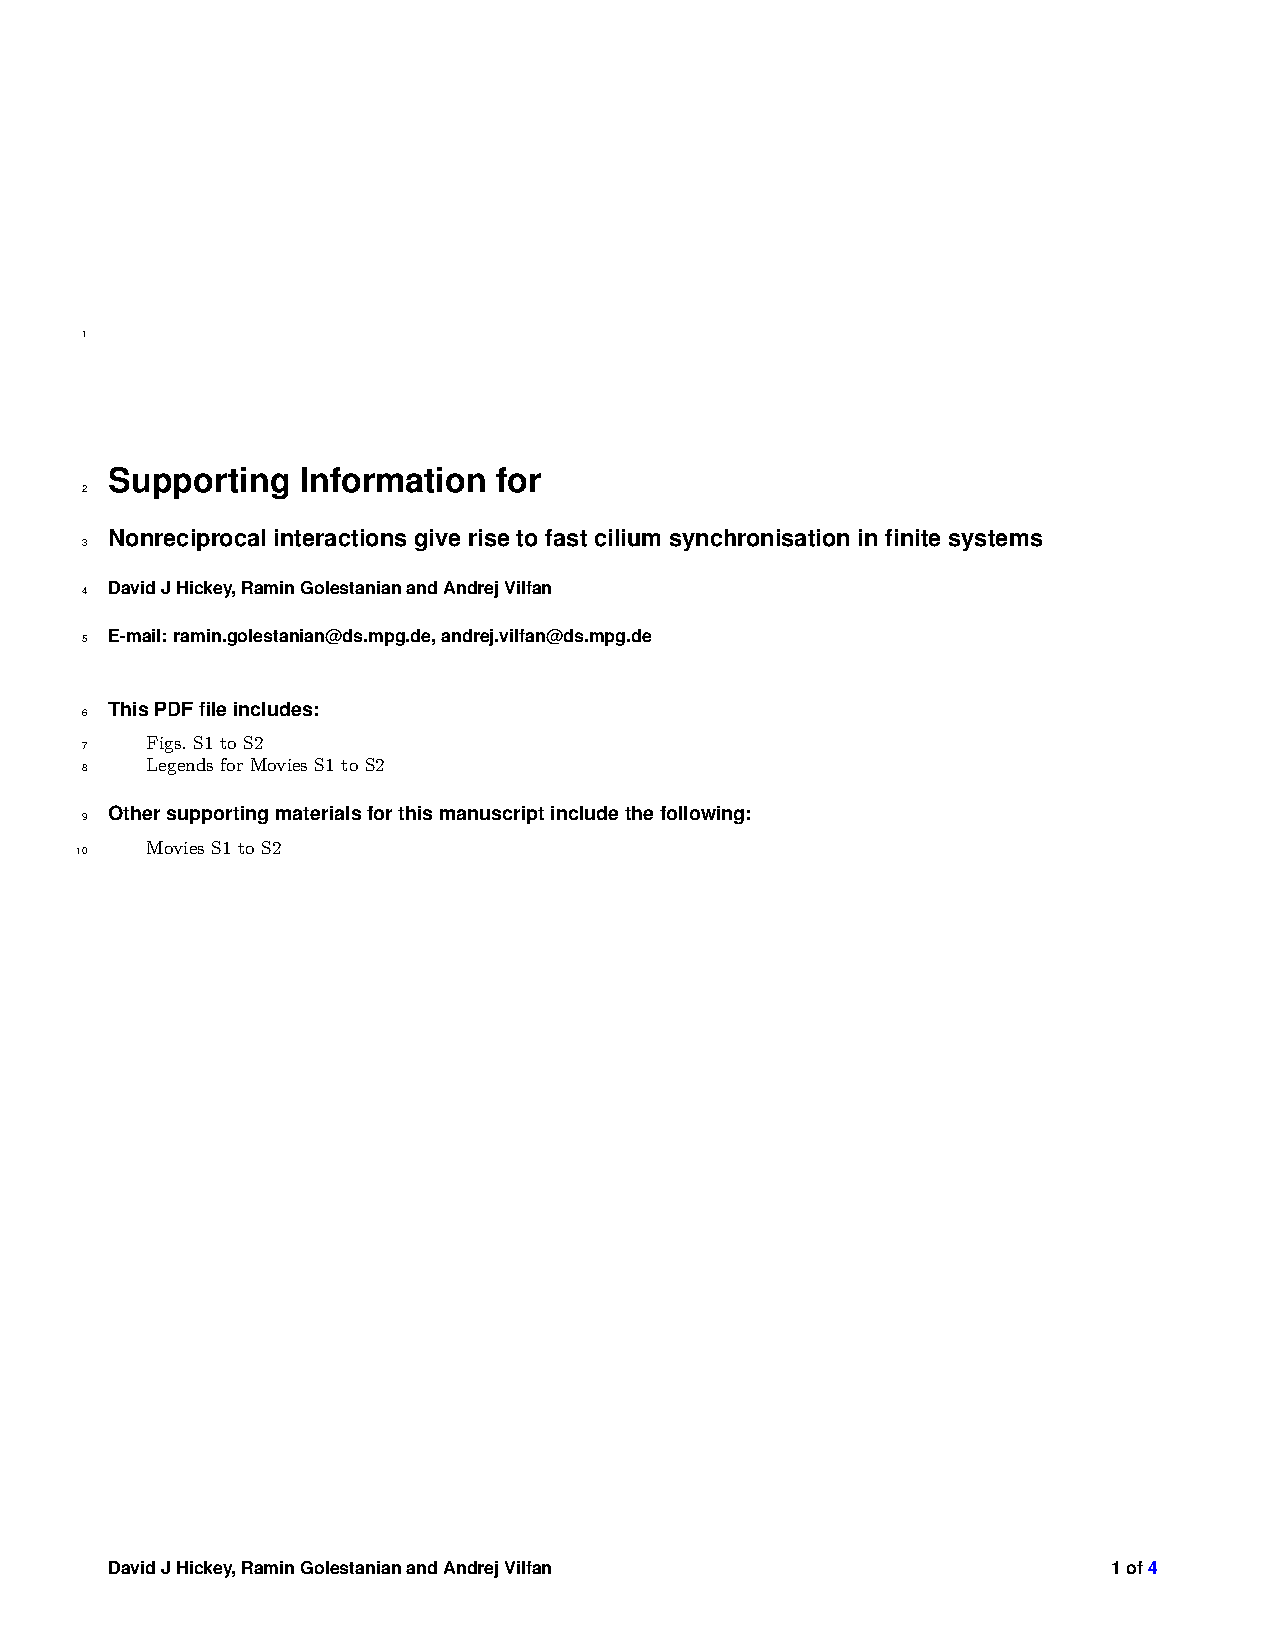
\includepdf[pages=-]{pdfs/Supplement___Nonreciprocal_Interactions____without_branding.pdf}

% As with the previous appendix
% \addtocontents{toc}{\protect\setcounter{tocdepth}{-1}}
% \chapter[Appendix C]{\phantom{X}}
% \addtocontents{toc}{\protect\setcounter{tocdepth}{\sectiontocdepth}}
% \addcontentsline{toc}{chapter}{Appendix C}
% \labch{appendixC}

% \hspace{0pt}
% \vfill
% \begin{fullwidth}
%     \section{List of figures}
% \end{fullwidth}
% \vfill
% \hspace{0pt}

% \listoffigures